\documentclass[11  pt]{exam} 
\usepackage[lmargin=1in,rmargin=1.75in,bmargin=1in,tmargin=1in]{geometry}  


% For hyperlinking everything
\usepackage{hyperref}
\hypersetup{
	colorlinks=true, %set true if you want colored links
	linktoc=all,     %set to all if you want both sections and subsections linked
	linkcolor=blue,  %choose some color if you want links to stand out
}


\usepackage[latin1]{inputenc}
\usepackage{amsmath}
\usepackage{mathrsfs}  
\usepackage{amsfonts}
\usepackage{amssymb}
\usepackage{graphicx}
\usepackage{subfig}
\usepackage{caption}
\usepackage{algorithm}
%\usepackage{algcompatible}
%\usepackage{algorithmicx}
\usepackage{algpseudocode}

\usepackage{titlesec}
\titleformat{\section}{\fontfamily{lmss}\fontsize{14}{15}\bfseries}{\thesection}{1em}{}
\titleformat{\subsection}{\fontfamily{lmss}\fontsize{12}{15}\bfseries}{\thesubsection}{1em}{}




\usepackage{amsthm}

\newtheoremstyle{noit}
{10pt}% <Space above>
{10pt}% <Space below>
{}% <Body font>
{}% <Indent amount>
{\bfseries}% <Theorem head font>
{.}% <Punctuation after theorem head>
{.5em}% <Space after theorem headi>
{}% <Theorem head spec (can be left empty, meaning `normal')>

\newtheoremstyle{example}
{10pt}% <Space above>
{10pt}% <Space below>
{}% <Body font>
{20pt}% <Indent amount>
{\bfseries}% <Theorem head font>
{.}% <Punctuation after theorem head>
{.5em}% <Space after theorem headi>
{}% <Theorem head spec (can be left empty, meaning `normal')>


\newtheoremstyle{indented}{20pt}{20pt}{\addtolength{\leftskip}{2.5em}}{}{\bfseries}{.}{.5em}{}


\newtheorem{theorem}{Theorem}
\numberwithin{theorem}{section}
\newtheorem{lemma}[theorem]{Lemma}
\newtheorem{corollary}[theorem]{Corollary}
\newtheorem{observation}{Observation}
%\numberwithin{observation}{section}
%\numberwithin{definition}{section}
\newtheorem{conjecture}{Conjecture}
\newtheorem{Qu}{Question}
\newcommand{\QU}{\begin{Qu}\normalfont}

\theoremstyle{noit}
\newtheorem{fact}{Fact}
\newtheorem{definition}{Definition}

\theoremstyle{indented}
\newtheorem{example}{Example}

\theoremstyle{indented}
\newtheorem{problem}{Problem}


%\newenvironment{proof}{\noindent{\bf Proof:} \hspace*{1em}}{
%    \hspace*{\fill} $\Box$ }
%\newenvironment{proof_of}[1]{\noindent {\bf Proof of #1:}
%    \hspace*{1em} }{\hspace*{\fill} $\Box$ }
%\newenvironment{proof_claim}{\begin{quotation} \noindent}{
%    \hspace*{\fill} $\diamond$ \end{quotation}}
\newcommand{\vs}[1]{\vspace{#1}}

\newcommand{\lecture}[2]{
 \noindent
\begin{center}
	\framebox{
		\vbox{
			\hbox to 5.78in { {\bf CSCE 411: Design and Analysis of Algorithms} \hfill  }
			\vspace{2mm}
			\hbox to 5.78in { {\Large \hfill Lecture #1\hfill} }
			\vspace{2mm}
			\hbox to 5.78in { {\it Date: #2 \hfill Lecturer: Nate Veldt} }
		}
	}
\end{center}
\vspace*{4mm}
}


\newcommand{\hw}[2]{
	\noindent
	\begin{center}
		\framebox{
			\vbox{
				\hbox to 5.78in { {\bf CSCE 411: Design and Analysis of Algorithms} \hfill  }
				\vspace{2mm}
				\hbox to 5.78in { {\Large \hfill Homework #1\hfill} }
				\vspace{2mm}
				\hbox to 5.78in { {\it Due date: #2 \hfil} }
			}
		}
	\end{center}
	\vspace*{4mm}
}



\newcommand{\under}[1]{\underline{\hspace{#1}}}
\setlength{\parindent}{0em}

%\usepackage[tagged]{accessibility}

% Graph terms
\newcommand{\vol}{\textbf{vol}}
\newcommand{\cut}{\textbf{cut}}


% Matrices
\newcommand{\mA}{\textbf{A}}
\newcommand{\mB}{\textbf{B}}

% vectors
\newcommand{\ve}{\textbf{e}}
\newcommand{\vx}{\textbf{x}}


% Other
\newcommand{\calN}{\mathcal{N}}

\usepackage{mathtools}
\DeclarePairedDelimiter\ceil{\lceil}{\rceil}
\DeclarePairedDelimiter\floor{\lfloor}{\rfloor}


\newcommand*{\aitem}{ \item[{
\includegraphics[width=0.8cm,height=0.5cm]{../../Lectures/figures/A}} ]  }
\newcommand*{\bitem}{ \item[{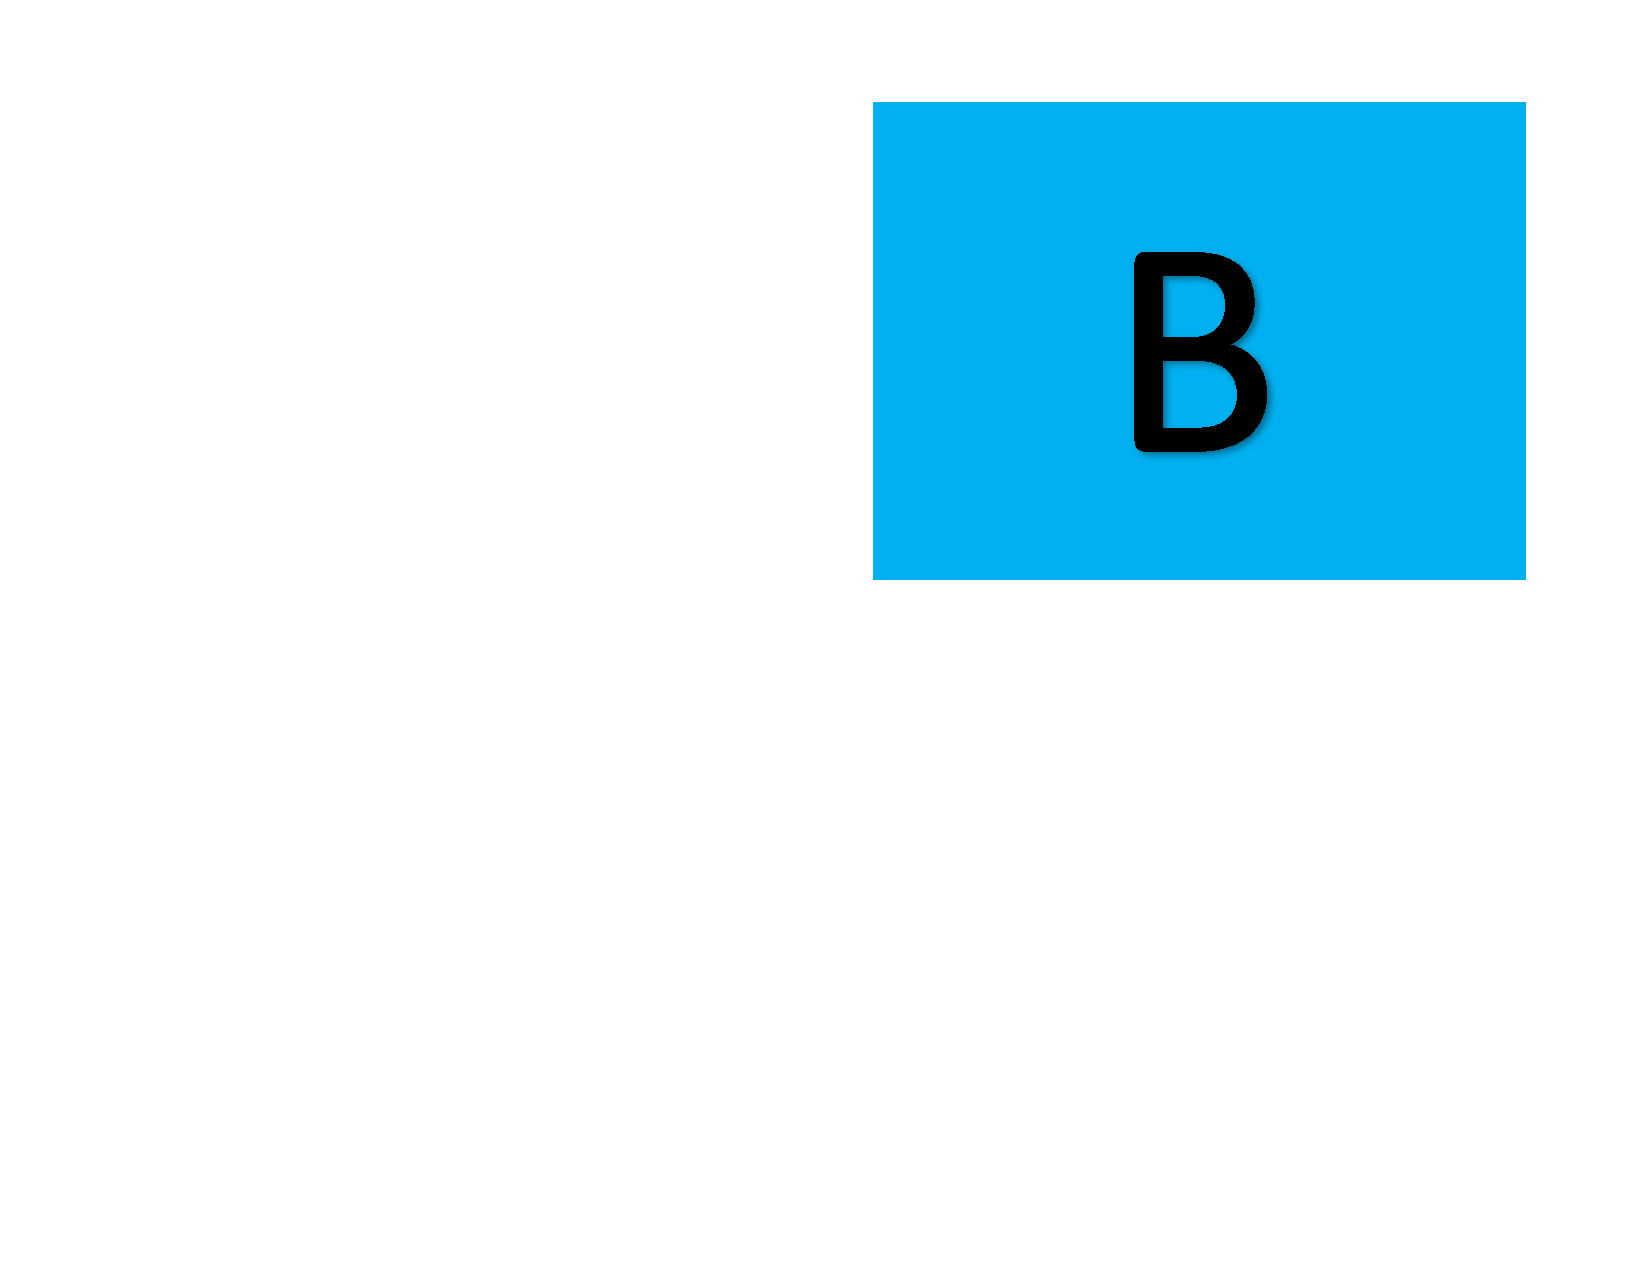
\includegraphics[width=0.8cm,height=0.5cm]{../../Lectures/figures/B}} ]  }
\newcommand*{\citem}{ \item[{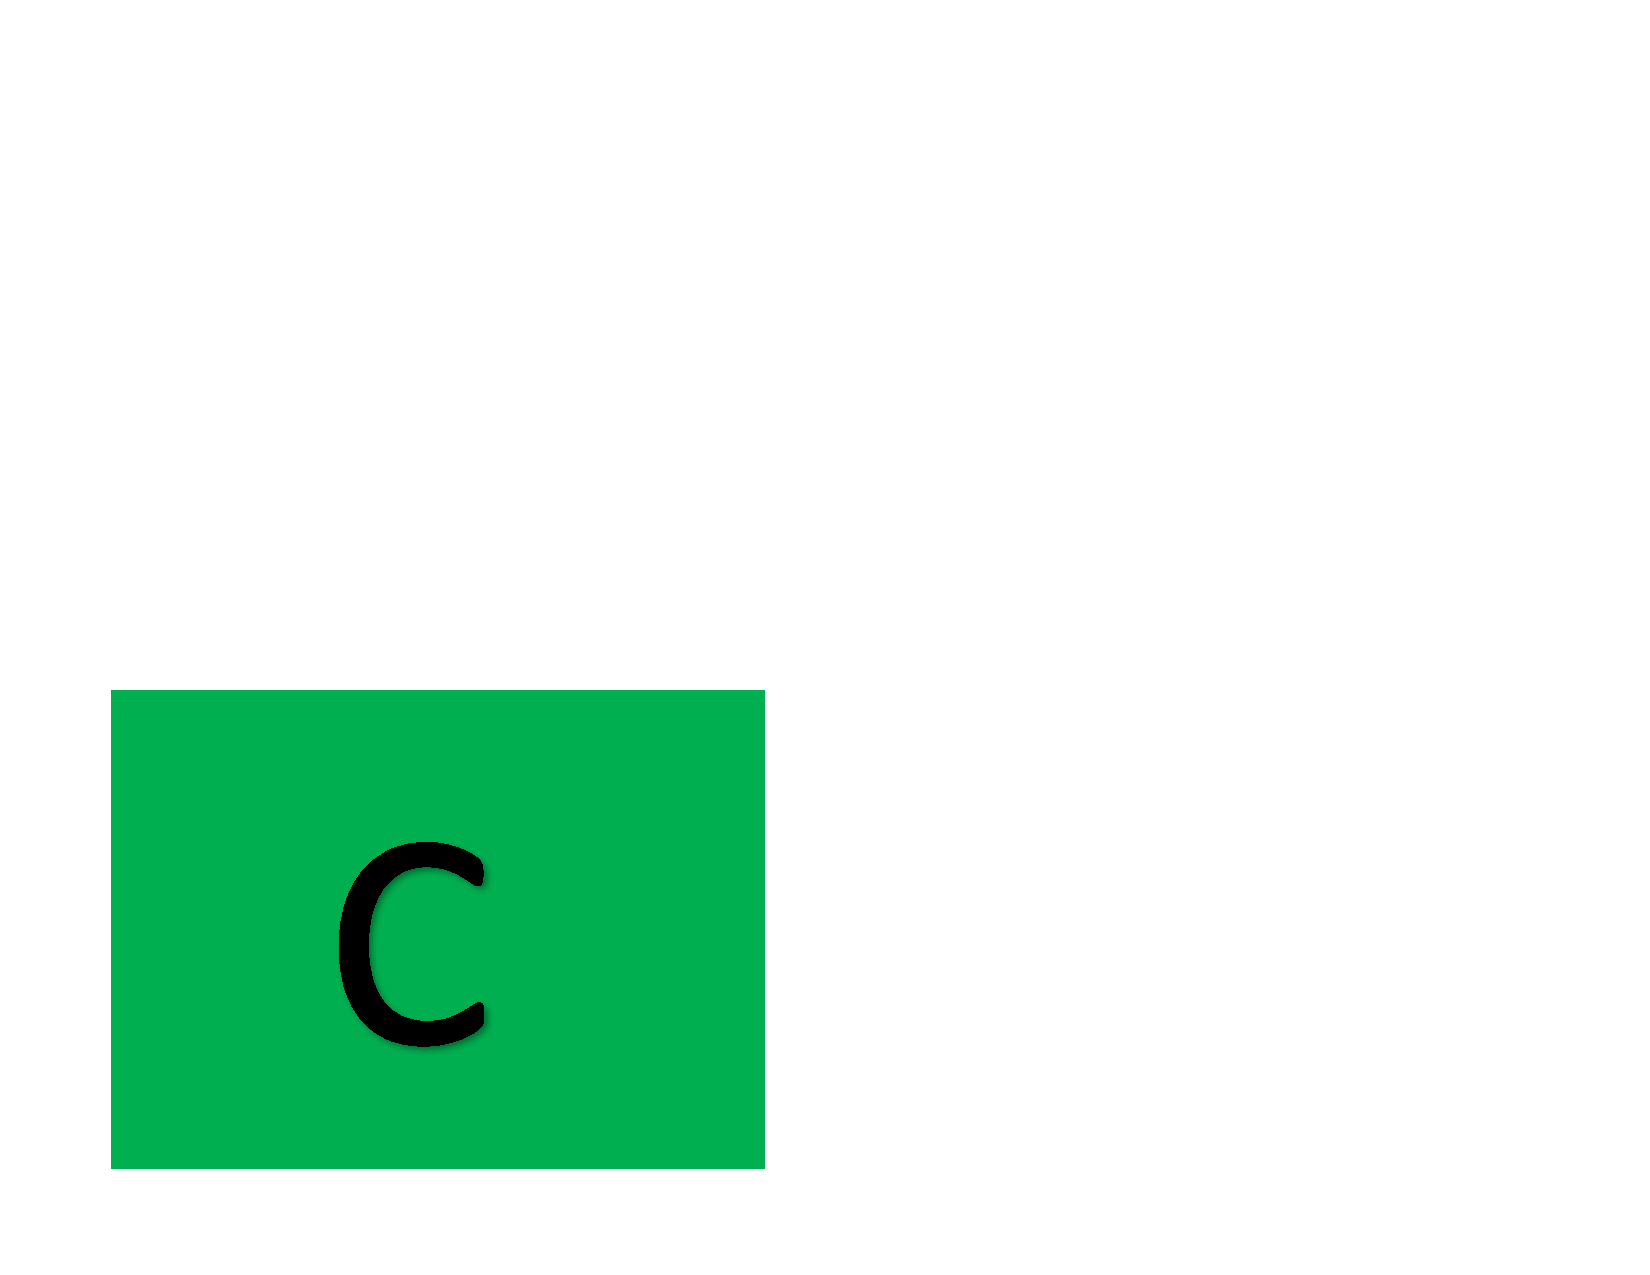
\includegraphics[width=0.8cm,height=0.5cm]{../../Lectures/figures/C}} ]  }
\newcommand*{\ditem}{ \item[{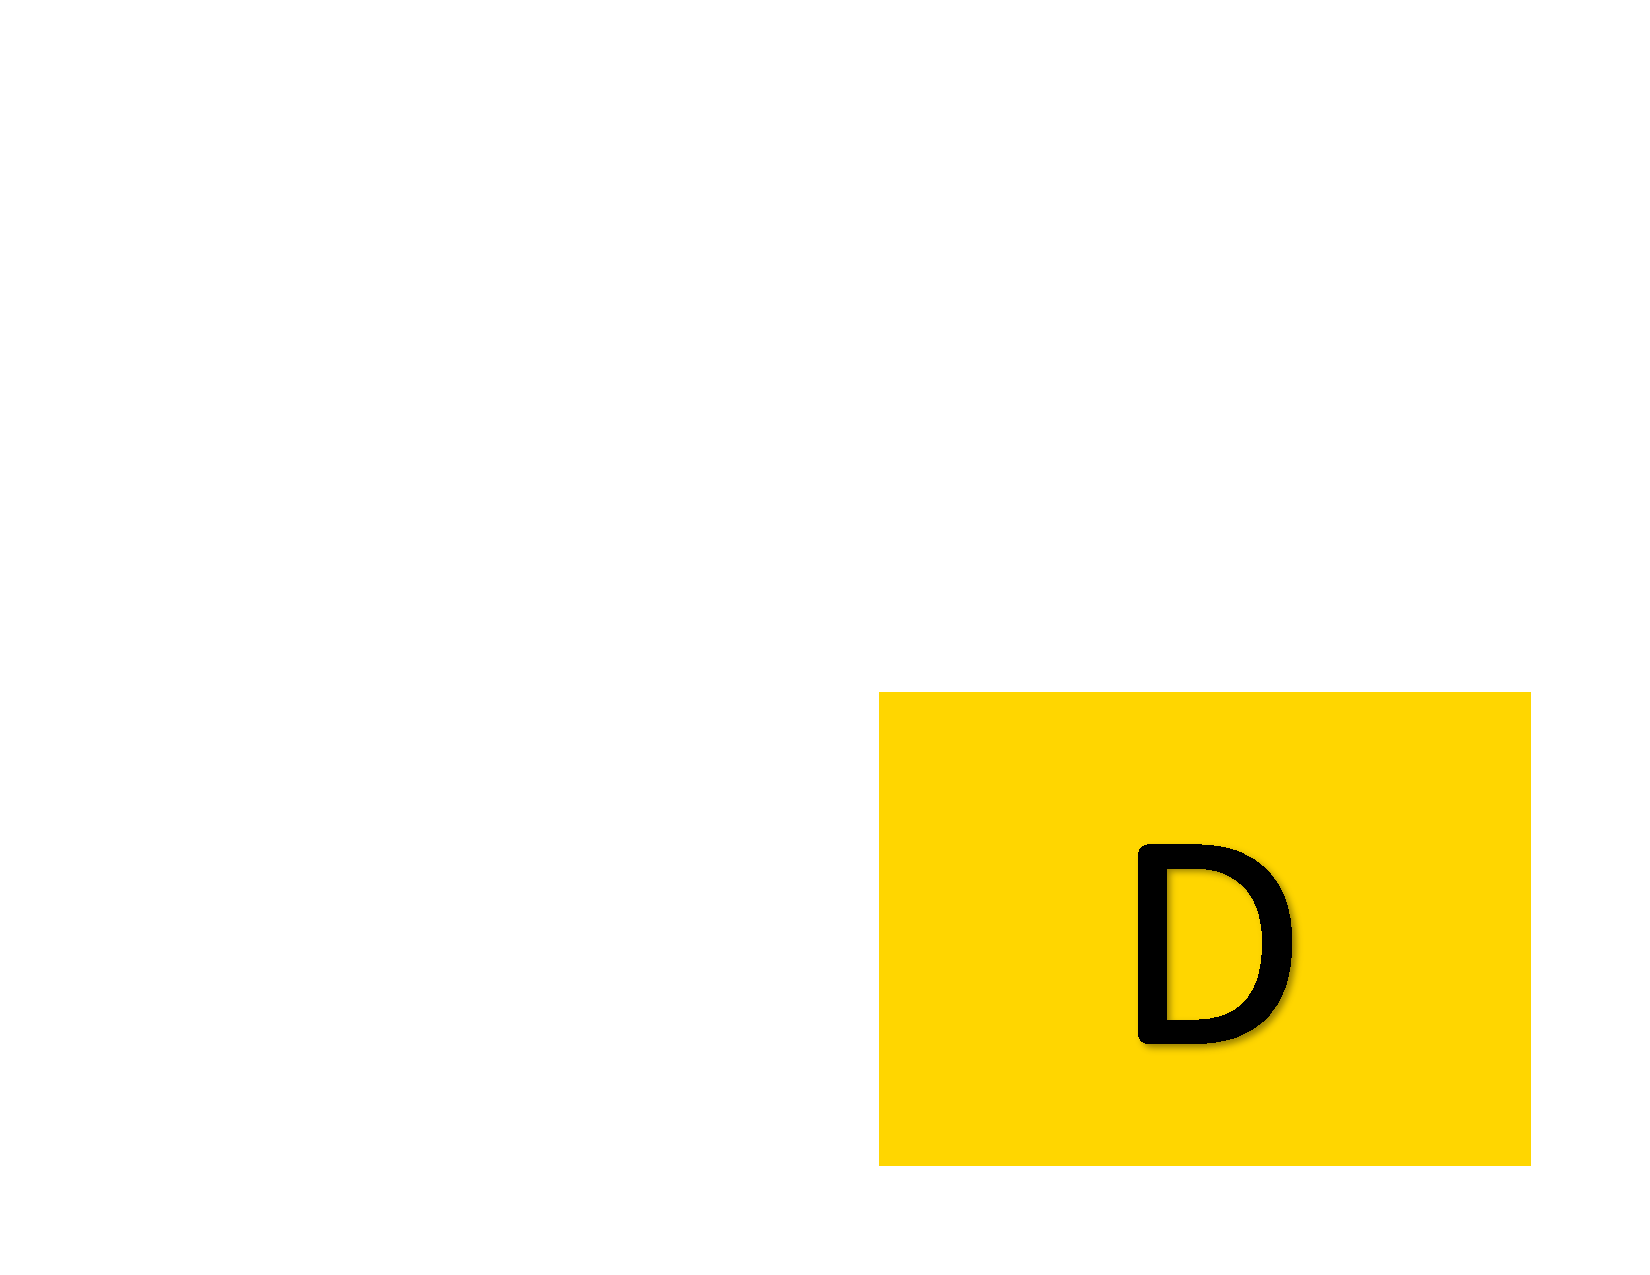
\includegraphics[width=0.8cm,height=0.5cm]{../../Lectures/figures/D}} ]  }
\newcommand*{\eitem}{ \item[{
\includegraphics[width=0.8cm,height=0.5cm]{../../Lectures/figures/E}} ]  }
\newcommand*{\fitem}{ \item[{
\includegraphics[width=0.8cm,height=0.5cm]{../../Lectures/figures/F}} ]  }


\newcommand{\hide}[1]{\underline{\phantom{#1 #1}}}

\usepackage{setspace}

\onehalfspacing

\begin{document}
	
	
	\begin{center}
		\framebox{
			\vbox{
				\hbox to 5.78in { {\bf CSCE 411: Design and Analysis of Algorithms} \hfill  }
				\vspace{2mm}
				\hbox to 5.78in { {\Large \hfill Final Exam Review \hfill} }
				\vspace{2mm}
				\hbox to 5.78in { {\it} }
			}
		}
	\end{center}
		

	\section{Test format and instructions}
	
	\begin{itemize}
		\item Some multiple choice questions, some long answer questions
		\item You do not need to prove something unless you are explicitly asked to prove something
		\item You may be asked to explicitly prove something 
		\item Scratch paper will be provided
		\item No calculators or electronic devices. You will not need them. If you have to do any computations, they will be basic enough to do by hand. 
		\item You will put your name on the front page, and put your initials at the top of every other page.
	\end{itemize}
	

	\emph{The basic format will be mostly the same as Tests 1 and 2, just longer. More multiple choice, and more free answer. }
	
	\begin{itemize}
		\item 15 multiple choice questions
		\item 4 free answer questions
	\end{itemize}

	\newpage
	

\section{What have we covered since Test 2 that you should know?}

\textbf{General concepts for complexity}
\begin{itemize}
	\item Definitions of: P, NP, NP-complete, NP-hard, and co-NP
	\item Understand basic open questions, e.g., P vs.\ NP
	\item What is required to prove something is in each of these problem classes
	\item What a reduction is, and what it means for it to be a polynomial time reduction
	\item How to use reductions to prove something is in P or in NP. (Make sure you understand how to beware of pitfalls in proving reductions!)
	\item There are some problems you should know are NP-complete: clique, graph coloring, vertex cover, clique cover, SAT, 3SAT, MAXCUT, subset sum, Hamiltonian path
	\item There are some problems you should know are in P: 2SAT, and pretty much all of the problems we covered before Test 2
\end{itemize}

\textbf{Reductions and problem we especially considered}
\begin{itemize}
	\item Graph clique and relationship with vertex cover
	%\item Graph coloring
	\item SAT, especially 2SAT and 3SAT
\end{itemize}

\textbf{Approximation algorithms and optimization}
\begin{itemize}
	\item You should know how to write a linear program and the dual linear program for an optimization problem
	\item You should know that there exist polynomial-time algorithms for solving linear programs
	\item Weak duality and strong duality theorems
\end{itemize}

\newpage
\section{What should I prioritize in my studying?}
What to study, roughly in the order I'd suggest you prioritize:
\begin{enumerate}
	\item The practice homework associated with the last week of lectures on NP-hardness reductions
	\item Practice problems at the end of this lecture
	\item The overview in these lecture notes
	\item Homeworks associated with last unit
	\item Study guides for Tests 1 and 2
	\item Everything else we covered during the course (lectures and homework)
\end{enumerate}

I suggest covering topics using a breadth first search rather than a depth first search. (Why preparation using depth first search can backfire: \url{https://xkcd.com/761/}).

\newpage


%\section{XKCD studying}
%If your study session is feeling a bit try, study concepts from class using XKCD comics:
%\begin{itemize}
%	\item DFS: \url{https://xkcd.com/761/}
%	\item DFS vs.\ BFS \url{https://xkcd.com/2407/}
%	\item NP-completeness \url{https://xkcd.com/287/}
%	\item Algorithmic complexity \url{https://xkcd.com/1667/}
%	\item Sorting algorithms \url{https://xkcd.com/1185/}
%	\item Traveling salesmen \url{https://xkcd.com/399/}
%\end{itemize}
	
	\section{Practice Problems}
	
	\begin{questions}
		
		\question 
		The decision problem of finding whether $G$ has a clique cover of size $k$ is denoted
		\begin{center}
			$\textsc{CliqueCover}(G,k) = \{ \langle G, k \rangle \colon \text{ determine if $G$ is has a clique cover of size $k$}\}$
		\end{center}
		
		% Variations: with planar graphs, you can color things, explain why this does not prove coloring is in P
		% Maxcut is hard: checking whether a graph is bipartite is easy
		
		(a) Prove that \textsc{CliqueCover} is in NP.
		
		(b) Prove that a graph $G = (V,E)$ has a $k$-coloring if and only if the complement graph $\bar{G} = (V, \bar{E})$ has a clique cover of size $k$.
		
		(c) Explain why the above fact implies that \textsc{CliqueCover} and \textsc{GraphColoring} are either both in $P$, or are both NP-complete.
		

	\question Bob is trying to prove that 2SAT can be reduced in polynomial time to the \textsc{Clique} problem. Do we already know whether this reduction is possible, or do we know for sure that it is impossible? Or is it an open question whether it is or isn't possible?  If he succeeds, what (if anything) will this tell us about the computational complexity of these problems? 
	
	\question Steve is trying to prove that every instance of 3SAT can be reduced in polynomial time to an instance of 2SAT.  Answer the same questions that you answered for problem 2.
	
	\question Alice is trying to come up with a polynomial time reduction from \textsc{Clique} to \textsc{MaxCut}. Answer the same questions that you answered for problem 2.
	
	\question Is the graph coloring problem NP-complete for general $k$? Is it still NP-complete when $k = 2$? Is it still NP-complete if $k = 3$?
	
	\question What is the difference between the class of NP-complete problems and the class of NP-hard problems? Are these classes exactly the same? If they are not exactly the same, explain how these two classes of problems differ.
	
	\question Susie says she came up with a polynomial time reduction from \textsc{Subset-Sum} to a new problem called \textsc{VertexHopping}. She explains to her friend Doug that this proves that the \textsc{VertexHopping} problem is NP-hard. Doug claims that this doesn't prove NP-hardness, because a problem is only NP-hard if \emph{every} problem in NP can be reduced to it, whereas Susie only proved that one specific problem in NP (\textsc{Subset-Sum}) can be reduced to \textsc{Vertex Hopping}. Is Doug right? If not, explain why he is wrong.

	
	\question Let $\textsc{MaxFlow}(G,s,t,k)$ represent the \emph{decision version} of the maximum $s$-$t$ flow problem where you are given a weighted directed graph with nodes $s$ and $t$ and the problem asks whether there is an $s$-$t$ flow function that sends $k$ units of flow from $s$ to $t$. Prove that this problem is in co-NP.
	
%	\question Let $\textsc{MinCut}(G,k)$ represent the following decision problem: check whether there is a way to separate the nodes of a graph $G$. Nevermind.
	
	\question A factory produces two drinks, $A$ and $B$. Each liter of product $A$ requires $2$ hours of labor and $1$ unit of raw material. Each liter of product $B$ requires $1$ hour of labor and $2$ units of raw material. The factory has a total of $100$ hours of labor and $80$ units of raw material available. The profit from each unit of product $A$ is $\$40$, and from each unit of product $B$ is $\$30$. The factory wants to maximize its total profit, assuming the amount of each drink produced does not need to be an integer. Write the linear program associated with this optimization problem. Write the dual linear program. 
	
\end{questions}
\end{document}
